%%
%% This is file `mcmthesis-demo.tex',
%% generated with the docstrip utility.
%%
%% The original source files were:
%%
%% mcmthesis.dtx  (with options: `demo')
%% !Mode:: "TeX:UTF-8"
%% -----------------------------------
%%
%% This is a generated file.
%%
%% Copyright (C)
%%     2010 -- 2015 by latexstudio
%%     2014 -- 2016 by Liam Huang
%%
%% This work may be distributed and/or modified under the
%% conditions of the LaTeX Project Public License, either version 1.3
%% of this license or (at your option) any later version.
%% The latest version of this license is in
%%   http://www.latex-project.org/lppl.txt
%% and version 1.3 or later is part of all distributions of LaTeX
%% version 2005/12/01 or later.
%%
%% This work has the LPPL maintenance status `maintained'.
%%
%% The Current Maintainer of this work is Liam Huang.
%%
\documentclass{mcmthesis}
\mcmsetup{CTeX = true,   % 使用 CTeX 套装时,设置为 true
        tcn = 1911507, problem = B,
        sheet = true, titleinsheet = true, keywordsinsheet = true,
        titlepage = false, abstract = true}
\usepackage{palatino}
\usepackage{lipsum}
\title{The \LaTeX{} Template for MCM Version \MCMversion}
\author{\small \href{http://www.latexstudio.net/}
  {
\includegraphics[width=7cm]{mcmthesis-logo}}}
\date{\today}
\begin{document}
\begin{abstract}
\lipsum[1]
\begin{keywords}
keyword1; keyword2
\end{keywords}
\end{abstract}
\maketitle
\tableofcontents
\newpage

\section{Model 1}
\noindent $X$: The number of the containers $X$.

\noindent $Y$: The number of the containers $Y$.

\noindent $Z$: The number of the containers $Z$.

\noindent $X_\alpha$: The number of the drones $\alpha$ packed in the container $X$.

\noindent $Y_\alpha$: The number of the drones $\alpha$ packed in the container $Y$.

\noindent $Z_\alpha$: The number of the drones $\alpha$ packed in the container $Z$.

\noindent $X_{\alpha ij}$: The number of the medical packages $i$ transported by drone $\alpha$ from container $X$'s location to the demand location $j$, where $\alpha=A,B,\cdots,H$, $i=1,2,3$, $j=1,2\cdots,5$.

\noindent $Y_{\alpha ij}$: The number of the medical packages $i$ transported by drone $\alpha$ from container $Y$'s location to the demand location $j$, where $\alpha=A,B,\cdots,H$, $i=1,2,3$, $j=1,2\cdots,5$.

\noindent $Z_{\alpha ij}$: The number of the medical packages $i$ transported by drone $\alpha$ from container $Z$'s location to the demand location $j$, where $\alpha=A,B,\cdots,H$, $i=1,2,3$, $j=1,2\cdots,5$.

\noindent $c_i$: The cost of the medical package $i$, where $i=1,2,3$.

\noindent $C_\alpha$: The cost of the drone $\alpha$, where $\alpha=A,B,\cdots,H$.

\noindent $W$: The cost of the container.

\noindent $V_\alpha$: The volume of the drone $\alpha$, where $\alpha=A,B,\cdots,H$.

\noindent $v_i$: The volume of the medical package $i$, where $i=1,2,3$.

\noindent $P_\alpha$: The max payload capability of the drone $\alpha$, where $\alpha=A,B,\cdots,H$.

\noindent $M$: A sufficiently large number for big-$M$ method in integer programming. 
\[
\begin{aligned}
&\min\quad\sum_{\alpha=A}^{H}\sum_{i=1}^{3}\sum_{j=1}^{5}c_{i}\left(X_{\alpha ij}+Y_{\alpha ij}+Z_{\alpha ij}\right)
+\sum_{\alpha=A}^{H}C_{{\alpha}}\left(X_{\alpha}+Y_{\alpha }+Z_{\alpha }\right)+W(X+Y+Z)\\
&\text{or}\\
&\max\quad d
\end{aligned}
\]
\[
\begin{aligned}
\text{s.t.}
\left\{
\begin{array}{lr}
\sum\limits_{i=1}^{3}\sum\limits_{j=1}^{5}v_{i}X_{\alpha ij}\le 8\times 10\times 14\ \text{ if }\alpha=A,B,D \\
\sum\limits_{i=1}^{3}\sum\limits_{j=1}^{5}v_{i}X_{\alpha ij}\le 24\times 20\times 20\ \text{ if }\alpha=C,E,F,G \\
\sum\limits_{i=1}^{3}\sum\limits_{j=1}^{5}v_{i}Y_{\alpha ij}\le 8\times 10\times 14\ \text{ if }\alpha=A,B,D \\
\sum\limits_{i=1}^{3}\sum\limits_{j=1}^{5}v_{i}Y_{\alpha ij}\le 24\times 20\times 20\ \text{ if }\alpha=C,E,F,G \\
\sum\limits_{i=1}^{3}\sum\limits_{j=1}^{5}v_{i}Z_{\alpha ij}\le 8\times 10\times 14\ \text{ if }\alpha=A,B,D \\
\sum\limits_{i=1}^{3}\sum\limits_{j=1}^{5}v_{i}Z_{\alpha ij}\le 24\times 20\times 20\ \text{ if }\alpha=C,E,F,G \\
\sum\limits_{\alpha=A}^{H}V_{\alpha}X_{\alpha}+\sum\limits_{\alpha=A}^{H}\sum\limits_{i=1}^{3}\sum\limits_{j=1}^{5}v_{i}X_{\alpha ij}\le 231\times92\times 94\\
\sum\limits_{\alpha=A}^{H}V_{\alpha}Y_{\alpha}+\sum\limits_{\alpha=A}^{H}\sum\limits_{i=1}^{3}\sum\limits_{j=1}^{5}v_{i}Y_{\alpha ij}\le 231\times92\times 94\\
\sum\limits_{\alpha=A}^{H}V_{\alpha}Z_{\alpha}+\sum\limits_{\alpha=A}^{H}\sum\limits_{i=1}^{3}\sum\limits_{j=1}^{5}v_{i}Z_{\alpha ij}\le 231\times92\times 94\\
\sum\limits_{i=1}^{3}\sum\limits_{j=1}^{5}X_{\alpha ij}\le M X_{\alpha}\ \text{ for }\alpha=A,B,\cdots, G\\
\sum\limits_{i=1}^{3}\sum\limits_{j=1}^{5}Y_{\alpha ij}\le M X_{\alpha}\ \text{ for }\alpha=A,B,\cdots, G\\
\sum\limits_{i=1}^{3}\sum\limits_{j=1}^{5}Z_{\alpha ij}\le M X_{\alpha}\ \text{ for }\alpha=A,B,\cdots, G\\
\sum\limits_{\alpha=A}^{H}X_\alpha\le MX\\
\sum\limits_{\alpha=A}^{H}Y_\alpha\le MY\\
\sum\limits_{\alpha=A}^{H}Z_\alpha\le MZ\\
X\le 1\\
Y\le 1\\
Z\le 1\\
\sum\limits_{j=1}^{5}\left(2X_{\alpha 1 j}+2X_{\alpha 2 j}+3X_{\alpha 3 j}\right)\le P_\alpha\text{ for }\alpha=A,B,\cdots, G\\
\sum\limits_{j=1}^{5}\left(2Y_{\alpha 1 j}+2Y_{\alpha 2 j}+3Y_{\alpha 3 j}\right)\le P_\alpha\text{ for }\alpha=A,B,\cdots, G\\
\sum\limits_{j=1}^{5}\left(2Z_{\alpha 1 j}+2Z_{\alpha 2 j}+3Z_{\alpha 3 j}\right)\le P_\alpha\text{ for }\alpha=A,B,\cdots, G\\
\end{array}
\right.
\end{aligned}
\]
\[
\begin{aligned}
\text{s.t.}&
\left\{
\begin{array}{lr}
\sum\limits_{\alpha=A}^{H}(X_{\alpha 11}+Y_{\alpha 11}+Z_{\alpha 11})\ge d\\
\sum\limits_{\alpha=A}^{H}(X_{\alpha 31}+Y_{\alpha 31}+Z_{\alpha 31})\ge d\\
\sum\limits_{\alpha=A}^{H}(X_{\alpha 12}+Y_{\alpha 12}+Z_{\alpha 12})\ge 2d\\
\sum\limits_{\alpha=A}^{H}(X_{\alpha 32}+Y_{\alpha 32}+Z_{\alpha 32})\ge d\\
\sum\limits_{\alpha=A}^{H}(X_{\alpha 13}+Y_{\alpha 13}+Z_{\alpha 13})\ge d\\
\sum\limits_{\alpha=A}^{H}(X_{\alpha 23}+Y_{\alpha 23}+Z_{\alpha 23})\ge d\\
\sum\limits_{\alpha=A}^{H}(X_{\alpha 14}+Y_{\alpha 14}+Z_{\alpha 14})\ge 2d\\
\sum\limits_{\alpha=A}^{H}(X_{\alpha 24}+Y_{\alpha 24}+Z_{\alpha 24})\ge d\\
\sum\limits_{\alpha=A}^{H}(X_{\alpha 34}+Y_{\alpha 34}+Z_{\alpha 34})\ge 2d\\
\sum\limits_{\alpha=A}^{H}(X_{\alpha 15}+Y_{\alpha 15}+Z_{\alpha 15})\ge d\\
X,Y,Z,X_\alpha,Y_\alpha,Z_\alpha,X_{\alpha ij},Y_{\alpha ij},Z_{\alpha ij} \text{ are nonnegative integers.}

\end{array}
\right.
\end{aligned}
\]

\section{Model 2: Maximizing Days}

\[
\begin{aligned}
\max\quad d
\end{aligned}
\]
\[
\begin{aligned}
\text{s.t.}
\left\{
\begin{array}{lr}
\sum\limits_{i=1}^{3}\sum\limits_{j=1}^{5}v_{i}X_{\alpha ij}\le 8\times 10\times 14\ \text{ if }\alpha=A,B,D \\
\sum\limits_{i=1}^{3}\sum\limits_{j=1}^{5}v_{i}X_{\alpha ij}\le 24\times 20\times 20\ \text{ if }\alpha=C,E,F,G \\
\sum\limits_{i=1}^{3}\sum\limits_{j=1}^{5}v_{i}Y_{\alpha ij}\le 8\times 10\times 14\ \text{ if }\alpha=A,B,D \\
\sum\limits_{i=1}^{3}\sum\limits_{j=1}^{5}v_{i}Y_{\alpha ij}\le 24\times 20\times 20\ \text{ if }\alpha=C,E,F,G \\
\sum\limits_{i=1}^{3}\sum\limits_{j=1}^{5}v_{i}Z_{\alpha ij}\le 8\times 10\times 14\ \text{ if }\alpha=A,B,D \\
\sum\limits_{i=1}^{3}\sum\limits_{j=1}^{5}v_{i}Z_{\alpha ij}\le 24\times 20\times 20\ \text{ if }\alpha=C,E,F,G \\
\sum\limits_{\alpha=A}^{H}V_{\alpha}X_{\alpha}+\sum\limits_{\alpha=A}^{H}\sum\limits_{i=1}^{3}\sum\limits_{j=1}^{5}v_{i}X_{\alpha ij}\le 231\times92\times 94\\
\sum\limits_{\alpha=A}^{H}V_{\alpha}Y_{\alpha}+\sum\limits_{\alpha=A}^{H}\sum\limits_{i=1}^{3}\sum\limits_{j=1}^{5}v_{i}Y_{\alpha ij}\le 231\times92\times 94\\
\sum\limits_{\alpha=A}^{H}V_{\alpha}Z_{\alpha}+\sum\limits_{\alpha=A}^{H}\sum\limits_{i=1}^{3}\sum\limits_{j=1}^{5}v_{i}Z_{\alpha ij}\le 231\times92\times 94\\
\sum\limits_{i=1}^{3}\sum\limits_{j=1}^{5}X_{\alpha ij}\le M X_{\alpha}\ \text{ for }\alpha=A,B,\cdots, G\\
\sum\limits_{i=1}^{3}\sum\limits_{j=1}^{5}Y_{\alpha ij}\le M X_{\alpha}\ \text{ for }\alpha=A,B,\cdots, G\\
\sum\limits_{i=1}^{3}\sum\limits_{j=1}^{5}Z_{\alpha ij}\le M X_{\alpha}\ \text{ for }\alpha=A,B,\cdots, G\\
\sum\limits_{\alpha=A}^{H}X_\alpha\le MX\\
\sum\limits_{\alpha=A}^{H}Y_\alpha\le MY\\
\sum\limits_{\alpha=A}^{H}Z_\alpha\le MZ\\
X\le 1\\
Y\le 1\\
Z\le 1\\
\sum\limits_{j=1}^{5}\left(2X_{\alpha 1 j}+2X_{\alpha 2 j}+3X_{\alpha 3 j}\right)\le P_\alpha\text{ for }\alpha=A,B,\cdots, G\\
\sum\limits_{j=1}^{5}\left(2Y_{\alpha 1 j}+2Y_{\alpha 2 j}+3Y_{\alpha 3 j}\right)\le P_\alpha\text{ for }\alpha=A,B,\cdots, G\\
\sum\limits_{j=1}^{5}\left(2Z_{\alpha 1 j}+2Z_{\alpha 2 j}+3Z_{\alpha 3 j}\right)\le P_\alpha\text{ for }\alpha=A,B,\cdots, G\\
\end{array}
\right.
\end{aligned}
\]
\[
\begin{aligned}
\text{s.t.}&
\left\{
\begin{array}{lr}
\sum\limits_{\alpha=A}^{H}X_{\alpha 11}\ge d\\
\sum\limits_{\alpha=A}^{H}X_{\alpha 31}\ge d\\
\sum\limits_{\alpha=A}^{H}X_{\alpha 12}\ge 2d\\
\sum\limits_{\alpha=A}^{H}X_{\alpha 32}\ge d\\
\sum\limits_{\alpha=A}^{H}X_{\alpha 13}\ge d\\
\sum\limits_{\alpha=A}^{H}X_{\alpha 23}\ge d\\
\sum\limits_{\alpha=A}^{H}X_{\alpha 14}\ge 2d\\
\sum\limits_{\alpha=A}^{H}X_{\alpha 24}\ge d\\
\sum\limits_{\alpha=A}^{H}X_{\alpha 34}\ge 2d\\
\sum\limits_{\alpha=A}^{H}X_{\alpha 15}\ge d\\
X,Y,Z,X_\alpha,Y_\alpha,Z_\alpha,X_{\alpha ij},Y_{\alpha ij},Z_{\alpha ij} \text{ are nonnegative integers.}

\end{array}
\right.
\end{aligned}
\]



\section{Model 2}
\[
\begin{aligned}
\min\quad&\sum_{\alpha=A}^{H}\sum_{i=1}^{3}\sum_{j=1}^{5}c_{i}\left(X_{\alpha ij}+Y_{\alpha ij}+Z_{\alpha ij}\right)
+\sum_{\alpha=A}^{H}C_{{\alpha}}\left(X_{\alpha}+Y_{\alpha }+Z_{\alpha }\right)+W(X+Y+Z)\\
&-R\sum_{k=1}^{K}\sum_{l=1}^{L}S_{kl}T_{kl}
\end{aligned}
\]
\[
\begin{aligned}
\text{s.t.}
\left\{
\begin{array}{lr}
\sum\limits_{i=1}^{3}\sum\limits_{j=1}^{5}v_{i}X_{\alpha ij}\le 8\times 10\times 14\ \text{ if }\alpha=A,B,D \\
\sum\limits_{i=1}^{3}\sum\limits_{j=1}^{5}v_{i}X_{\alpha ij}\le 24\times 20\times 20\ \text{ if }\alpha=C,E,F,G \\
\sum\limits_{i=1}^{3}\sum\limits_{j=1}^{5}v_{i}Y_{\alpha ij}\le 8\times 10\times 14\ \text{ if }\alpha=A,B,D \\
\sum\limits_{i=1}^{3}\sum\limits_{j=1}^{5}v_{i}Y_{\alpha ij}\le 24\times 20\times 20\ \text{ if }\alpha=C,E,F,G \\
\sum\limits_{i=1}^{3}\sum\limits_{j=1}^{5}v_{i}Z_{\alpha ij}\le 8\times 10\times 14\ \text{ if }\alpha=A,B,D \\
\sum\limits_{i=1}^{3}\sum\limits_{j=1}^{5}v_{i}Z_{\alpha ij}\le 24\times 20\times 20\ \text{ if }\alpha=C,E,F,G \\
\sum\limits_{\alpha=A}^{H}V_{\alpha}X_{\alpha}+\sum\limits_{\alpha=A}^{H}\sum\limits_{i=1}^{3}\sum\limits_{j=1}^{5}v_{i}X_{\alpha ij}\le 231\times92\times 94\\
\sum\limits_{\alpha=A}^{H}V_{\alpha}Y_{\alpha}+\sum\limits_{\alpha=A}^{H}\sum\limits_{i=1}^{3}\sum\limits_{j=1}^{5}v_{i}Y_{\alpha ij}\le 231\times92\times 94\\
\sum\limits_{\alpha=A}^{H}V_{\alpha}Z_{\alpha}+\sum\limits_{\alpha=A}^{H}\sum\limits_{i=1}^{3}\sum\limits_{j=1}^{5}v_{i}Z_{\alpha ij}\le 231\times92\times 94\\
\sum\limits_{i=1}^{3}\sum\limits_{j=1}^{5}X_{\alpha ij}\le M X_{\alpha}\ \text{ for }\alpha=A,B,\cdots, G\\
\sum\limits_{i=1}^{3}\sum\limits_{j=1}^{5}Y_{\alpha ij}\le M X_{\alpha}\ \text{ for }\alpha=A,B,\cdots, G\\
\sum\limits_{i=1}^{3}\sum\limits_{j=1}^{5}Z_{\alpha ij}\le M X_{\alpha}\ \text{ for }\alpha=A,B,\cdots, G\\
\sum\limits_{\alpha=A}^{H}X_\alpha\le MX\\
\sum\limits_{\alpha=A}^{H}Y_\alpha\le MY\\
\sum\limits_{\alpha=A}^{H}Z_\alpha\le MZ\\
X\le 1\\
Y\le 1\\
Z\le 1\\
\sum\limits_{j=1}^{5}\left(2X_{\alpha 1 j}+2X_{\alpha 2 j}+3X_{\alpha 3 j}\right)\le P_\alpha\text{ for }\alpha=A,B,\cdots, G\\
\sum\limits_{j=1}^{5}\left(2Y_{\alpha 1 j}+2Y_{\alpha 2 j}+3Y_{\alpha 3 j}\right)\le P_\alpha\text{ for }\alpha=A,B,\cdots, G\\
\sum\limits_{j=1}^{5}\left(2Z_{\alpha 1 j}+2Z_{\alpha 2 j}+3Z_{\alpha 3 j}\right)\le P_\alpha\text{ for }\alpha=A,B,\cdots, G\\
\end{array}
\right.
\end{aligned}
\]
\[
\begin{aligned}
\text{s.t.}&
\left\{
\begin{array}{lr}
\sum\limits_{\alpha=A}^{H}X_{\alpha 11}\ge d\\
\sum\limits_{\alpha=A}^{H}X_{\alpha 31}\ge d\\
\sum\limits_{\alpha=A}^{H}X_{\alpha 12}\ge 2d\\
\sum\limits_{\alpha=A}^{H}X_{\alpha 32}\ge d\\
\sum\limits_{\alpha=A}^{H}X_{\alpha 13}\ge d\\
\sum\limits_{\alpha=A}^{H}X_{\alpha 23}\ge d\\
\sum\limits_{\alpha=A}^{H}X_{\alpha 14}\ge 2d\\
\sum\limits_{\alpha=A}^{H}X_{\alpha 24}\ge d\\
\sum\limits_{\alpha=A}^{H}X_{\alpha 34}\ge 2d\\
\sum\limits_{\alpha=A}^{H}X_{\alpha 15}\ge d\\
X,Y,Z,X_\alpha,Y_\alpha,Z_\alpha,X_{\alpha ij},Y_{\alpha ij},Z_{\alpha ij} \text{ are nonnegative integers.}

\end{array}
\right.
\end{aligned}
\]
\section{Introduction}

\lipsum[2]
\begin{itemize}
\item minimizes the discomfort to the hands, or
\item maximizes the outgoing velocity of the ball.
\end{itemize}
We focus exclusively on the second definition.

\begin{itemize}
\item the initial velocity and rotation of the ball,
\item the initial velocity and rotation of the bat,
\item the relative position and orientation of the bat and ball, and
\item the force over time that the hitter hands applies on the handle.
\end{itemize}
\lipsum[3]
\begin{itemize}
\item the angular velocity of the bat,
\item the velocity of the ball, and
\item the position of impact along the bat.
\end{itemize}
\lipsum[4]
\emph{center of percussion} [Brody 1986], \lipsum[5]

\begin{Theorem} \label{thm:latex}
\LaTeX
\end{Theorem}
\begin{Lemma} \label{thm:tex}
\TeX .
\end{Lemma}
\begin{proof}
The proof of theorem.
\end{proof}

\subsection{Other Assumptions}
\lipsum[6]
\begin{itemize}
\item
\item
\item
\item
\end{itemize}

\lipsum[7]

\section{Analysis of the Problem}
\begin{figure}[h]
\small
\centering
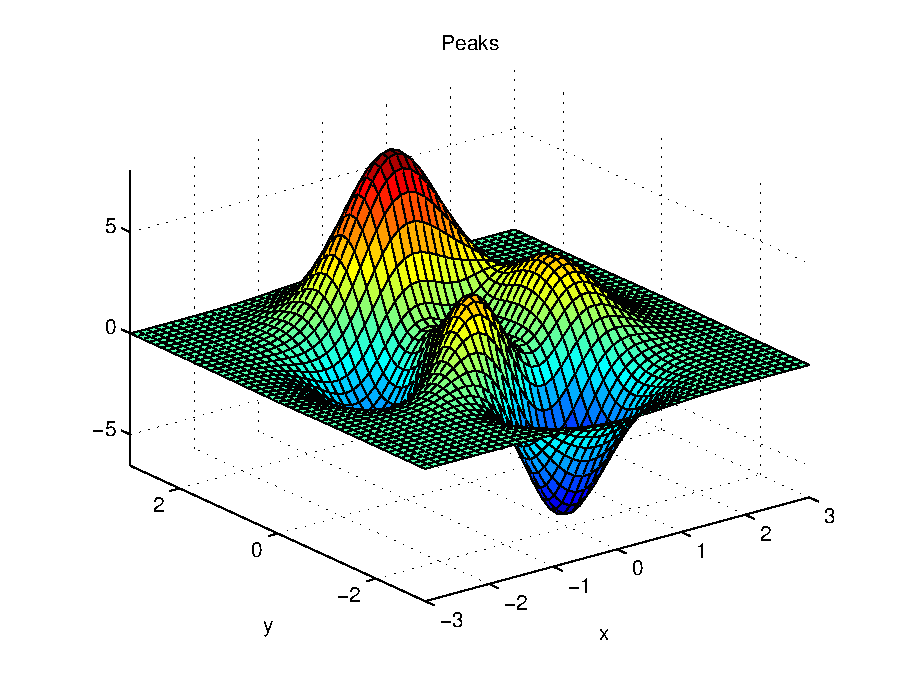
\includegraphics[width=12cm]{mcmthesis-aaa.eps}
\caption{aa} \label{fig:aa}
\end{figure}

\lipsum[8] \eqref{aa}
\begin{equation}
a^2 \label{aa}
\end{equation}

\[
  \begin{pmatrix}{*{20}c}
  {a_{11} } & {a_{12} } & {a_{13} }  \\
  {a_{21} } & {a_{22} } & {a_{23} }  \\
  {a_{31} } & {a_{32} } & {a_{33} }  \\
  \end{pmatrix}
  = \frac{{Opposite}}{{Hypotenuse}}\cos ^{ - 1} \theta \arcsin \theta
\]
\lipsum[9]

\[
  p_{j}=\begin{cases} 0,&\text{if $j$ is odd}\\
  r!\,(-1)^{j/2},&\text{if $j$ is even}
  \end{cases}
\]

\lipsum[10]

\[
  \arcsin \theta  =
  \mathop{{\int\!\!\!\!\!\int\!\!\!\!\!\int}\mkern-31.2mu
  \bigodot}\limits_\varphi
  {\mathop {\lim }\limits_{x \to \infty } \frac{{n!}}{{r!\left( {n - r}
  \right)!}}} \eqno (1)
\]

\section{Calculating and Simplifying the Model  }
\lipsum[11]

\section{The Model Results}
\lipsum[6]

\section{Validating the Model}
\lipsum[9]

\section{Conclusions}
\lipsum[6]

\section{A Summary}
\lipsum[6]

\section{Evaluate of the Mode}

\section{Strengths and weaknesses}
\lipsum[12]

\subsection{Strengths}
\begin{itemize}
\item \textbf{Applies widely}\\
This  system can be used for many types of airplanes, and it also
solves the interference during  the procedure of the boarding
airplane,as described above we can get to the  optimization
boarding time.We also know that all the service is automate.
\item \textbf{Improve the quality of the airport service}\\
Balancing the cost of the cost and the benefit, it will bring in
more convenient  for airport and passengers.It also saves many
human resources for the airline. \item \textbf{}
\end{itemize}

\begin{thebibliography}{99}
\bibitem{1} D.~E. KNUTH   The \TeX{}book  the American
Mathematical Society and Addison-Wesley
Publishing Company , 1984-1986.
\bibitem{2}Lamport, Leslie,  \LaTeX{}: `` A Document Preparation System '',
Addison-Wesley Publishing Company, 1986.
\bibitem{3}\url{http://www.latexstudio.net/}
\bibitem{4}\url{http://www.chinatex.org/}
\end{thebibliography}

\begin{appendices}

\section{First appendix}

\lipsum[13]

Here are simulation programmes we used in our model as follow.\\

\textbf{\textcolor[rgb]{0.98,0.00,0.00}{Input matlab source:}}
\lstinputlisting[language=Matlab]{./code/mcmthesis-matlab1.m}

\section{Second appendix}

some more text \textcolor[rgb]{0.98,0.00,0.00}{\textbf{Input C++ source:}}
\lstinputlisting[language=C++]{./code/mcmthesis-sudoku.cpp}

\end{appendices}
\end{document}

%%
%% This work consists of these files mcmthesis.dtx,
%%                                   figures/ and
%%                                   code/,
%% and the derived files             mcmthesis.cls,
%%                                   mcmthesis-demo.tex,
%%                                   README,
%%                                   LICENSE,
%%                                   mcmthesis.pdf and
%%                                   mcmthesis-demo.pdf.
%%
%% End of file `mcmthesis-demo.tex'.
